% Suffix trie, suffix tree, and implicit suffix tree for cabab, left to right.
% Regenerate from this directory:
% latex -interaction=nonstopmode -halt-on-error suffix-tree1.tex
% dvisvgm --no-fonts --exact --bbox=papersize -o suffix-tree1.svg suffix-tree1.dvi
\documentclass[tikz,border=8pt]{standalone}
\usepackage{lmodern}
\begin{document}
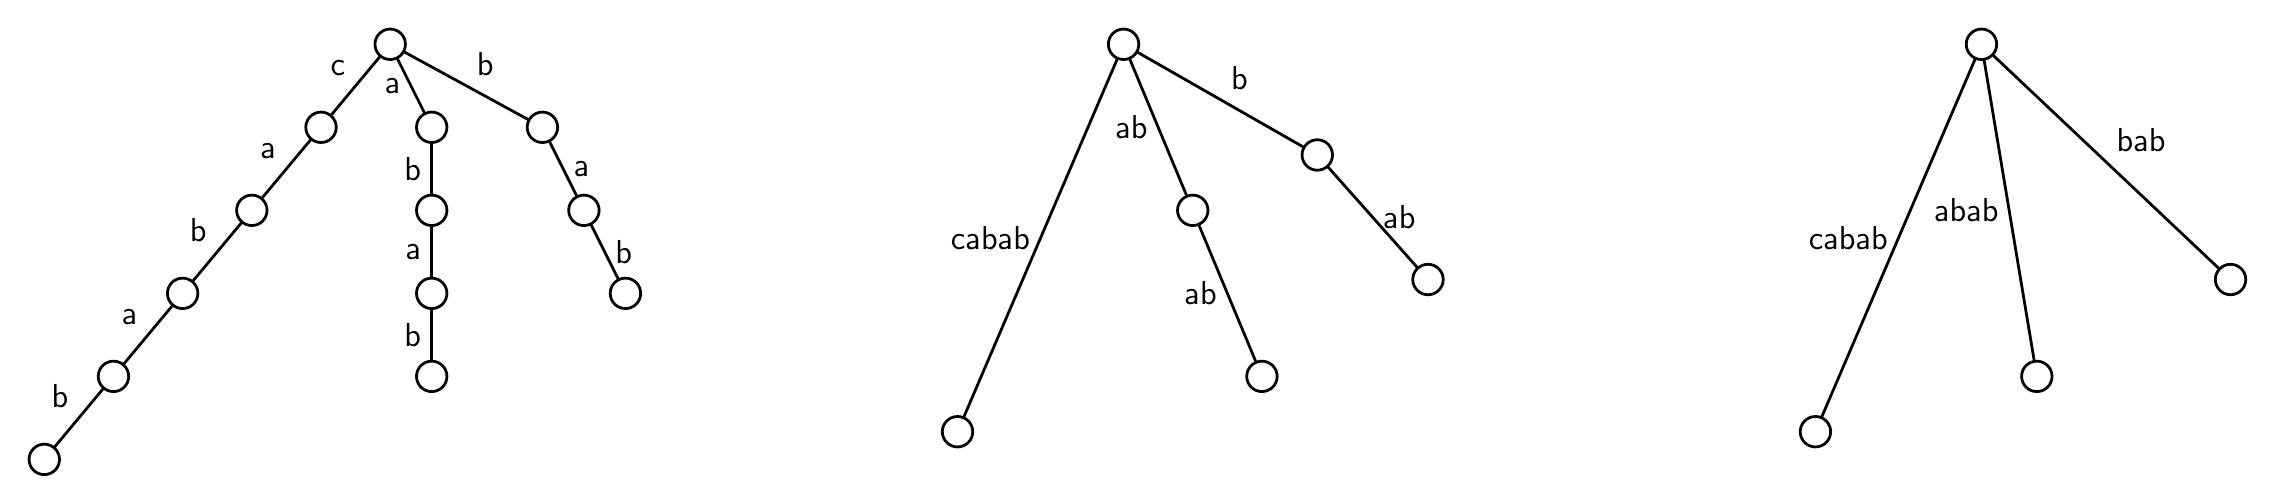
\begin{tikzpicture}[
  x=1pt,y=-1pt,line width=1pt,line cap=round,
  font=\sffamily\fontsize{12}{14}\selectfont,
  vertex/.style={circle,draw,fill=white,minimum size=11pt,inner sep=0pt},
  every edge/.style={draw}
]
  % The uncompressed trie has one edge per character.
  \node[vertex] (trie-root) at (125,0) {};
  \node[vertex] (trie-c) at (100,30) {};
  \node[vertex] (trie-ca) at (75,60) {};
  \node[vertex] (trie-cab) at (50,90) {};
  \node[vertex] (trie-caba) at (25,120) {};
  \node[vertex] (trie-cabab) at (0,150) {};
  \node[vertex] (trie-a) at (140,30) {};
  \node[vertex] (trie-ab) at (140,60) {};
  \node[vertex] (trie-aba) at (140,90) {};
  \node[vertex] (trie-abab) at (140,120) {};
  \node[vertex] (trie-b) at (180,30) {};
  \node[vertex] (trie-ba) at (195,60) {};
  \node[vertex] (trie-bab) at (210,90) {};
  \path
    (trie-root) edge node[above left] {c} (trie-c)
    (trie-c) edge node[above left] {a} (trie-ca)
    (trie-ca) edge node[above left] {b} (trie-cab)
    (trie-cab) edge node[above left] {a} (trie-caba)
    (trie-caba) edge node[above left] {b} (trie-cabab)
    (trie-root) edge node[left] {a} (trie-a)
    (trie-a) edge node[left] {b} (trie-ab)
    (trie-ab) edge node[left] {a} (trie-aba)
    (trie-aba) edge node[left] {b} (trie-abab)
    (trie-root) edge node[above right] {b} (trie-b)
    (trie-b) edge node[right] {a} (trie-ba)
    (trie-ba) edge node[right] {b} (trie-bab);

  % Keep every suffix endpoint when compressing the trie.
  \node[vertex] (tree-root) at (390,0) {};
  \node[vertex] (tree-cabab) at (330,140) {};
  \node[vertex] (tree-ab) at (415,60) {};
  \node[vertex] (tree-abab) at (440,120) {};
  \node[vertex] (tree-b) at (460,40) {};
  \node[vertex] (tree-bab) at (500,85) {};
  \path
    (tree-root) edge node[left] {cabab} (tree-cabab)
    (tree-root) edge node[left] {ab} (tree-ab)
    (tree-ab) edge node[left] {ab} (tree-abab)
    (tree-root) edge node[above right] {b} (tree-b)
    (tree-b) edge node[right] {ab} (tree-bab);

  % Suppress the degree-one suffix endpoints ab and b in the implicit tree.
  \node[vertex] (implicit-root) at (700,0) {};
  \node[vertex] (implicit-cabab) at (640,140) {};
  \node[vertex] (implicit-abab) at (720,120) {};
  \node[vertex] (implicit-bab) at (790,85) {};
  \path
    (implicit-root) edge node[left] {cabab} (implicit-cabab)
    (implicit-root) edge node[left] {abab} (implicit-abab)
    (implicit-root) edge node[above right] {bab} (implicit-bab);
\end{tikzpicture}
\end{document}
